% !TeX root=../main.tex

\chapter{مروری بر مطالعات انجام شده}
%\thispagestyle{empty} 
\section{مقدمه}
این فصل به مروری بر برخی از مهم‌ترین روش‌های موجود در حوزه کشف تقلب می‌پردازد. در ابتدا دسته‌بندی کلی برای حل مسئله کشف تقلب ارائه می‌شود و سپس دامنه تمرکز روی یک شاخه از این روش‌ها محدود می‌گردد. هرچند که امروزه استفاده از روش‌های یادگیری عمیق گسترش فراوان یافته است و در بسیاری از مسائل بینایی ماشین، روش‌های کلاسیک منسوخ شده‌اند؛ اما این از اهمیت روش‌های کلاسیک نمی‌کاهد.
روش‌های کلاسیک بینایی ماشین در مقایسه با روش‌های مبتنی بر یادگیری عمیق، از آنجا که تمرکز بیشتری روی الگوریتم تا تمرکز روی استفاده از داده داشته‌اند، می‌توانند دید میدانی خوبی از نزدیک شدن به مسئله بدهند.


در این پایان‌نامه سعی شده است که از این دید کلاسیک برای حل مسئله با بهره گرفتن از ابزارهای یادگیری عمیق استفاده شود. پس در این فصل ابتدا روش‌های کلاسیک مورد بررسی قرار می‌گیرند و سپس مروری بر روش‌های مبتنی بر یادگیری عمیق انجام می‌گیرد. 
همانطور که در شکل 
\ref{fig:algs}
مشخص است روش کلی الگوریتم‌های کشف تقلب و به‌طور کلی بسیاری از مسائل بینایی ماشین ابتدا استخراج ویژگی از تصویر یا ویدیوی ورودی است و سپس طبقه‌بندی ویژگی‌های به‌دست آمده است. استخراج ویژگی نقش مهمی در دقت طبقه‌بندی خواهد داشت. یک استخراج ویژگی، یک تابع از تصویر ورودی به یک بردار است و زمانی استخراج ویژگی به‌درستی انجام گرفته است که بردار خروجی شامل اطلاعات اساسی و مهم برای طبقه‌بندی صحیح باشد.

تفاوت عمده الگوریتم‌های کلاسیک و یادگیری عمیق در قسمت استخراج ویژگی است. بدین صورت که در روش‌های کلاسیک، ویژگی‌ها با استفاده از یک روش ایستا انتخاب می‌شوند ولی در روش‌های شبکه عصبی عمیق با استفاده از بهینه‌سازی یک تابع هزینه، روی داده‌های آموزش، استخراج ویژگی‌های مد نظر یاد گرفته می‌شوند.

\begin{figure}[ht]
\begin{tikzpicture}
	\tikzstyle{connection}=[ultra thick,every node/.style={sloped,allow upside down},draw=\edgecolor,opacity=0.7]
	\node[canvas is zy plane at x=0] (temp) at (-3,0,0)
	{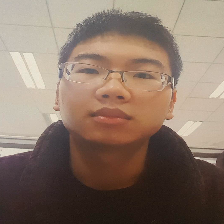
\includegraphics[width=2cm,height=2cm]{1_1_09_2f_37.png}};
	
	\draw [color=black]
	(temp) node[anchor=south] at (-3,-2){\texttt{Input Face}};
	%\draw[connection] 
	\draw[->,thick] (-2.5,0) -- (-2,0);
	
	\node[trapezium,
	draw = blue!80,
	text = black,
	fill = teal!20,
	rotate=270,
	trapezium stretches = true,
	minimum width = 2cm, 
	minimum height = 3cm] (t) at (-.5,0) {Feature Extraction};
	
	\draw[->,thick] (1.2,0) -- (1.7,0);
	
	\node[rectangle,
	draw = magenta!80,
	text = black,
	fill = magenta!20,
	rotate=270,
	trapezium stretches = true,
	minimum width = 2cm, 
	minimum height = 2cm] (t) at (3,0) {Classification};
	
	%\pic[shift={(1.5,0,0)}] at (4,0) {Ball={name=elt1,%
	%		fill=\SumColor,opacity=0.6,%
	%		radius=3,logo=1/0?}};
	
\end{tikzpicture}
\caption{ساختار کلی الگوریتم‌های کشف تقلب در چهره}
\label{fig:algs}
\end{figure}

در روش‌های کلاسیک، با استفاده از الگوریتم‌های بینایی ماشین، سعی در یافتن یک مؤلفه‌ی مفید از تصویر است که به یافتن علائم مربوط به تقلب در تصویر کمک کند. روش‌های کلاسیک به دو دسته سخت‌افزاری و نرم‌افزاری تقسیم می‌شوند.
\cite{ramachandra2017presentation}


در روش‌های سخت‌افزاری یا از یک سخت افزار خاص استفاده می‌شود، یا از یک تعامل فیزیکی با کاربر نظیر چشمک زدن و یا پاسخ به یک چالش استفاده می‌گردد.
در حالت استفاده از سخت افزار خاص، یک دوربین حرارتی یا چند طیفی به کار برده می‌شود. در این حالت تمایز بین تصویر صورت واقعی و یک کاغذ از طریق بررسی طیف نوری یا حرارت مشخص می‌گردد. در حالت‌های دیگر از کاربر خواسته می‌شود یک سری کلمات را ادا کرده1 یا با دست خود حرکت خاصی را انجام دهد.
لازم به ذکر است که در روش‌های سخت افزاری، قسمت نرم‌افزار حذف نمی‌شود و پردازش‌ها به‌صورت خاص متناسب با سخت‌افزار در خواهند آمد. این بدین معنی است که استفاده از سخت‌افزار، طراحی الگوریتم را حذف نخواهد کرد، بلکه نوع الگوریتم، خاص منظوره بر اساس سخت‌افزار مورد استفاده خواهد شد.
مشکل روش‌های سخت‌افزاری این است که هزینه اضافی دارد و تعامل بیشتر کاربر با سیستم را تحمیل می‌کند. تعامل بیشتر، زمان احراز هویت را طولانی‌تر می‌کند که مطلوب نیست.


در روش‌های نرم‌افزاری از سخت افزار اضافه‌ای استفاده نمی‌شود؛ و تنها از همان دوربین معمولی، تصویربرداری صورت می‌گیرد؛ اما از یک الگوریتم هوشمند بر پایه‌ی بینایی ماشین استفاده خواهد شد. روش‌های نرم‌افزاری به دو دسته ایستان و پویا تقسیم می‌شود.
در روش‌های ایستان، پردازش تنها روی یک فریم تصویر انجام می‌شود و تقلب را با اطلاعات تک تصویر بررسی می‌کند؛ هر چند که این روش‌ها را در دنباله ویدیویی نیز می‌توان به کار برد و روی هر فریم، این پردازش صورت بگیرد. این روش‌ها هزینه محاسباتی کمتری در مقایسه با روش‌های پویا دارند. روش‌های ایستان به سه دسته تحلیل ریزبافت1، تحلیل فرکانس و روش ترکیبی تقسیم می‌شود.
در تحلیل ریزبافت از الگوهای بافت تصویر استفاده می‌شود. این الگوها در مقیاس ذره بینی بررسی می‌گردند. معروف‌ترین عملگر برای این تحلیل عملگر الگوهای دودویی محلی2 (LBP) است که با جزئیات در ادامه توضیح خواهد داده شد.
در روش تحلیل فرکانسی بر اساس تبدیل فوریه و تحلیل مولفه‌های فرکانسی صورت می‌گیرد و شامل استفاده از فیلتر تفاضلی گوسی و تبدیل کسینوسی می‌شود.
در روش‌های پویا از اطلاعات فریم‌های متوالی نیز در کنار هم استفاده می‌شود و برای تحلیل، وابستگی فریم‌های متوالی بررسی می‌شود. در مقایسه با روش‌های ایستان زمان پردازش بیشتری دارند اما دقت بهتری را ارائه می‌کنند. روش‌های پویا به سه دسته تحلیل حرکت، تحلیل بافت و روش‌های ترکیبی تقسیم می‌شود.
در روش پویا از حرکت عضلات صورت به‌وسیله حرکت سر، دهان و چشم بهره برده می‌شود. الگوریتم‌های مورد استفاده در این در بیشتر موارد بر مبنای الگوریتم optical flow است. همچنین روش‌های جداسازی صورت از پس‌زمینه و اطلاعات فرکانسی متحرک نیز مورد استفاده قرار می‌گیرد. همچنین از تغییرات بافت در بین فریم‌های متوالی استفاده می‌شود.
\section{تحلیل ریز بافت و عملگر LBP}
در میان روش‌های نرم‌افزاری ذکر شده، تحلیل ریزبافت در این پایان‌نامه اهمیت بسزایی دارد. یکی از تفاوت‌های بین تصویر واقعی و تقلبی در بررسی بافت اجزای صورت در مقیاس ذره‌بینی1 است. در این مقیاس اثر دانه دانه‌ای چاپ تصویر روی کاغذ منجر به تفاوت با بافت طبیعی چهره انسان نمایان می‌شود. همچنین صورت انسان در مقایسه با تصویر نمایش داده شده روی نمایشگر دیجیتال از نظر بافت پیکسلی متفاوت خواهد بود. همچنین صورت واقعی در مقایسه با تصویر چاپ شده یا نشان داده شده روی نمایشگر دیجیتال از نظر انعکاس نور و بازتاب و تشکیل سایه تفاوت دارد. علاوه بر این‌ها تصاویر تقلبی در مجموع کمی تاری در کیفیت خود دارند. از این رو مسئله کشف تقلب، شباهت‌هایی با مسائل تحلیل کیفیت تصاویر و نهان‌کاوی دارد.

در 
\cite{maatta2011face}
برای اولین بار از عملگر الگوهای دودویی محلی یا به اختصار LBP، در حوزه کشف تقلب در چهره استفاده شده است. این عملگر از تعریف بافت از در یک همسایگی در مقیاس محلی الهام گرفته است و یک توصیف‌گر قوی بافت است. به‌منظور آشنایی اولیه، این عملگر ابتدا در یک پنجره سه در سه تعریف می‌شود و سپس رابطه محاسبه آن به‌صورت کلی تعریف می‌شود. در شکل 
\ref{fig:lbpexm}
مثالی از محاسبه این عملگر در پنجره سه در سه نشان داده شده است.
\begin{figure}[ht]
	\centerline{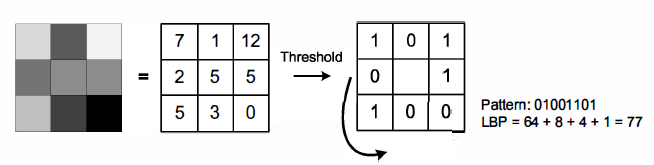
\includegraphics[width=\linewidth]{lbpexm}}
	\caption{مثالی از محاسبه LBP }
	\label{fig:lbpexm}
\end{figure}
ابتدا پیکسل‌های کناری با پیکسل میانی مقایسه می‌شوند، سپس بر مبنای بزرگ‌تر یا کوچک‌تر بودن مقادیر از پیکسل میانی مقدار یک یا صفر به آنها اختصاص داده می‌شود و سپس این دنباله دودویی در یک جهت دایره‌ای خوانده و یک عدد هشت بیتی می‌دهد. در پنجره سه در سه 8 پیکسل مجاور موجود هست و تعداد حالت‌هایی که خروجی عملگر می‌تواند داشته باشد برابر با
$2^8=256$
است.





تعریف رسمی این عملگر به‌صورت کلی برای شعاع R و تعداد نقاط نمونه برداری P در محیط دایره به‌صورت رابطه
\ref{eq:lbpDef}
است.
\begin{equation}\label{eq:lbpDef}
			LBP_{P,R}=\sum_{p=0}^{P-1}s(I_p-I_c)2^p 
\end{equation}

که در آن
$s(.)$
یک تابع غیر خطی است.

\[ s(x) = 
\begin{cases} 1  & \text{$x \geq 0 $}\,; \\
	0  & \text{otherwise}\,.
\end{cases} \]

این رابطه بیان می‌کند برای محاسبه ریزبافت هر پیکسل در هر نقطه ابتدا یک دایره به شعاع R در نظر گرفته و روی محیط آن P نقطه به فواصل مساوی باید انتخاب شود. در صورتی که برخی نقاط انتخاب شده روی پیکسل خاصی قرار نگیرد باید با استفاده از درون‌یابی دو خطی1، مقدار پیکسلی به آن تخصیص داده شود. سپس مقدار این پیکسل‌های روی دایره با پیکسل مرکز دایره مقایسه شده و دنباله دودویی ایجاد می‌گردد. این عمل بدین صورت ادامه می‌یابد که مرکز دایره لغزانده شده و هر بار برای هر پیکسل تصویر ورودی، مقدار LBP محاسبه می‌گردد.

یکی از ویژگی‌های مهم این عملگر، مقاوم بودن در برابر تغییرات یکسان پیکسل‌های تصویر ورودی است. فرض کنید تمامی پیکسل‌ها در یک عدد ثابت ضرب شده یا با یک مقدار ثابت جمع شوند در این صورت به‌علت اینکه خروجی تابع غیرخطی تغییر نخواهد کرد مقدار نهایی خروجی LBP تغییری نمی‌کند.
همچنین این عملگر بار محاسباتی کمی دارد پس سریع است. تفاضل گیریی و اعمال تابع غیر خطی   
$s(.)$
ساده است و اعمال ضریب
$2^p$
به کمک شیفت، قابل انجام است.
\begin{align}\label{eq:lbpfeature}
	&I \to \alpha I \to s(\alpha I_p -\alpha I_c) = s(I_p - I_c) \\
	&I \to I+\beta \to s((I_p + \beta)-(I_c + \beta)) = s(I_p - I_c ) 
\end{align}

یک نسخه تکامل یافته از LBP، نسخه‌ی یکنواخت این عملگر است که با  نشان داده می‌شود. این عملگر از این رو معرفی شده است که برخی از الگوهای دودویی بیشتر از سایرین در تصویر متداول‌اند. یک LBP را یکنواخت گویند اگر حداکثر دو تغییر از صفر به یک یا برعکس در نمایش دودویی آن به‌صورت چرخشی وجود داشته باشد. برای محاسبه برچسب خروجی در حالت یکنواخت، هر الگوی یکنواخت با یک مقدار مجزا نشان داده می‌شود و تمامی حالت‌های غیر یکنواخت به یک مقدار متناظر می‌شوند.

هر خروجی LBP می‌تواند نمایانگر وجود یک نوع الگوی ریزبافت باشد. برای مثال یک LBP با مقدار خاص می‌تواند نشانگر نقطه، گوشه، مسطح و... باشد. پس فراوانی این الگوها در تصویر اهمیت دارد. پس از محاسبه LBP به ازای هر پیکسل تصویر، هیستوگرام آن محاسبه می‌شود و از طریق توزیع فراوانی الگوهای ریزبافت‌های متفاوت موجود در تصویر، در مورد واقعی یا غیر واقعی بودن آن تصمیم گیری می‌شود.
\begin{figure}[hb]
	\centerline{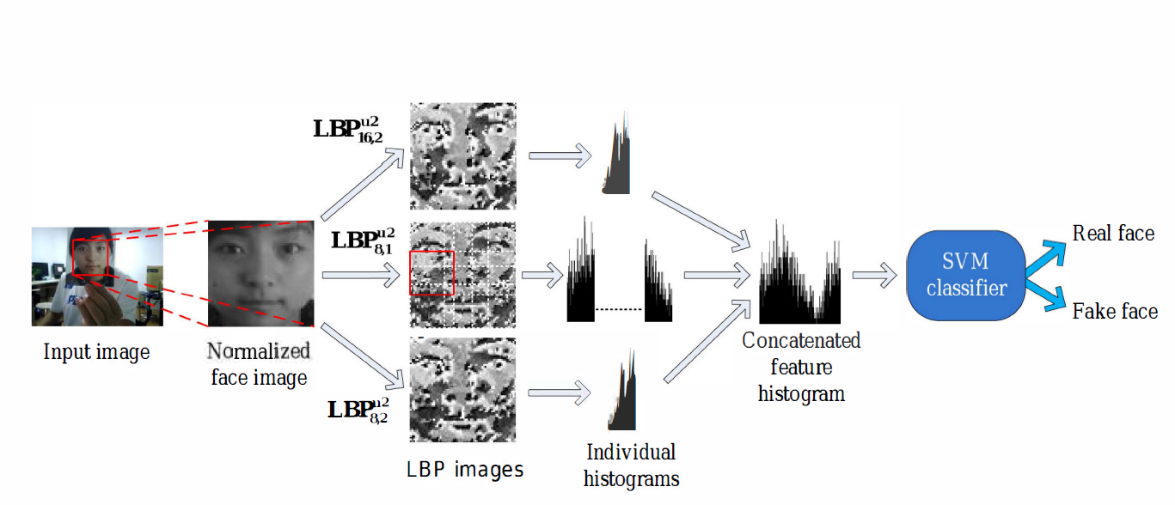
\includegraphics[width=\linewidth]{lbpmatta}}
	\caption{روش تصمیم‌گیری بر اساس استفاده از LBP \cite{maatta2011face}}
	\label{fig:lbpmatta}
\end{figure}

روش محاسبه و تصمیم گیری ارائه شده در 
\cite{maatta2011face}
در مورد واقعی یا تقلبی بودن تصویر چهره با استفاده از تحلیل ریزبافت به‌صورت شکل
\ref{fig:lbpmatta}
است.
ابتدا با استفاده از الگوریتم تشخیص چهره، مختصات صورت انتخاب شده و مقادیر پیکسلی چهره به‌صورت نرمالیزه می‌شود. سپس عملگر LBP با شعاع‌های متفاوت اعمال شده و هیستوگرام آنها محاسبه می‌شود، سپس این هیستوگرام‌ها کنار هم گذاشته می‌شود و با الگوریتم SVM طبقه بندی صورت می‌گیرد.

در 
\cite{chingovska2012effectiveness}
بر خلاف روش قبلی تنها از عملگر LBP یکنواخت در پنجره سه در سه به‌صورت نرمالیزه شده استفاده شده است و از عملگر LBP با شعاع‌های متنوع 
\cite{maatta2011face}
استفاده نشده است. همچنین در 
\cite{chingovska2012effectiveness}
به این نکته پرداخته شده است که باید به ریزبافت در نواحی مختلف صورت توجه داشت و توزیع فراوانی ریزبافت‌ها را نباید صرفاً در کل ناحیه صورت بررسی کرد.
\begin{figure}[t]
	\centerline{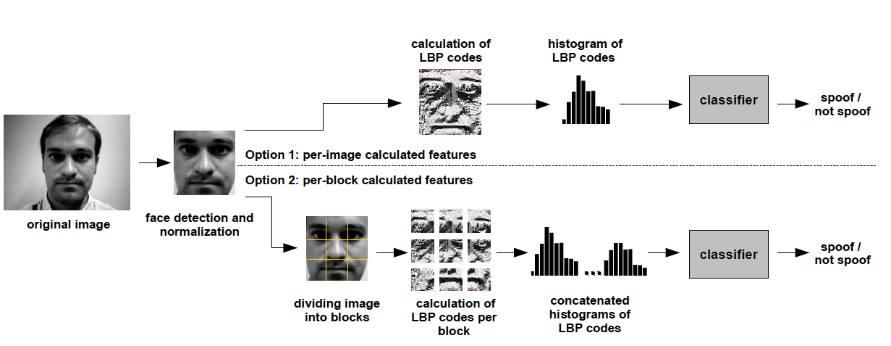
\includegraphics[width=\linewidth]{lbpchin}}
	\caption{روش تحلیل ریزبافت در نواحی مختلف تصویر \cite{chingovska2012effectiveness}}
	\label{fig:lbpchin}
\end{figure}
در این روش در یک حالت هیستوگرام LBP صورت در کل تصویر محاسبه می‌شود؛ در حالت دیگر ناحیه صورت به 9 ناحیه تقسیم شده و در هر کدام به‌صورت جداگانه هیستوگرام LBP محاسبه می‌شود و این هیستوگرام‌ها در کنار هم قرار داده می‌شود. سپس هیستوگرام‌ها به‌عنوان یک بردار ویژگی به طبقه‌بند داده می‌شود. در این روش توزیع هر تصویر با توزیع هیستوگرام تصویر چهره واقعی مقایسه می‌شود این مقایسه به روش X2 histogram comparison انجام می‌گیرد.

دو روش گفته شده از LBP به‌صورت ایستا استفاده کرده‌اند. یعنی ورودی سیستم تنها یک تصویر از چهره فرد است. از آنجا که اطلاعات بین فریم‌ها یعنی تحلیل یک دنباله ویدیویی، می‌تواند به دقت تشخیص کمک کند، پریریا و همکاران عملگر LBP را در فضای سه‌بعدی گسترش داده‌اند تا از اطلاعات بافت در حوزه مکانی تصویر و حوزه زمانی بین فریم‌های متوالی در تصمیم‌گیری استفاده شود
\cite{freitas2012lbp}.
\section{روش‌های مبتنی بر یادگیری عمیق}
 در عملگر LBP انتخاب ویژگی به‌صورت دستی انجام می‌گیرد. انگیزه انتخاب ویژگی به‌صورت هوشمند موجب استفاده از روش‌های یادگیری عمیق برای این کار شده است. ایده استفاده از یادگیری عمیق در حوزه کشف تقلب در تشخیص چهره برای اولین بار توسط ینگ و همکاران مطرح شد 
\cite{yang2014learn}
.
 روش ارائه شده در این کار بدین صورت است که ابتدا صورت تشخیص داده می‌شود و پنجره انتخاب شده برای صورت، به‌گونه‌ای در مقیاس‌های مختلف بزرگ می‌شود که شامل پس زمینه صورت نیز باشد. چرا که اطلاعات پس زمینه نیز می‌تواند به کشف تقلب کمک کند. سپس این تصاویر به یک شبکه ALEXNET
\cite{krizhevsky2012imagenet}
  داده می‌شود و این شبکه کانولوشن ویژگی‌های مد نظر را استخراج می‌کند و در انتها به‌وسیله SVM طبقه‌بندی صورت می‌گیرد.با اینکه این کار در سال 2014 انجام شده است، اما کاشف به عمل آمده است که استفاده خام از شبکه عصبی عمیق به تنهایی نمی‌تواند به دقت مطلوب برسد. به همین دلیل تاکنون پژوهش‌ها در این حوزه ادامه داشته است و ایده‌های مختلفی برای بهبود عملکرد و افزایش دقت طبقه‌بندی مطرح شده است. 
 
 روش گفته شده روی یک فریم کار می‌کند. برای بهره بردن از اطلاعات بین فریم‌های مختلف استفاده از کانولوشن سه بعدی پیشنهاد شده است 
\cite{gan20173d,li2018learning}
 . شیوه دیگر برای کمک گرفتن اطلاعات فریم‌های متوالی استفاده از ساختار
LSTM \cite{hochreiter1997long}
  پس از شبکه کانولوشن است که کارهای
\cite{xu2015learning,yang2019face}
از این ساختار استفاده کرده‌اند.
 

\subsection{ترکیب روش‌های یادگیری عمیق و ویژگی‌های دستی}
یک ایده برای افزایش دقت شبکه عصبی پیشنهاد ترکیب ویژگی‌های لایه‌های کانولوشن با ویژگی‌های دستی1 است. نمای کلی حالت مختلفی که می‌توان برای این کار، ساختار ارائه کرد در شکل 
\ref{fig:cnn-hand}
نشان داده شده است 
\cite{yu2021deep}
 حالت‌های مخلتف این روش بدین صورت است که می‌توان ابتدا ویژگی دستی را استخراج کرد و این ویژگی‌ها را به یک شبکه عمیق داد. یا می‌توان ابتدا از شبکه عمیق برای استخراج ویژگی استفاده کرد و سپس روی ویژگی‌های عمیق به‌دست آمده از روش‌های استخراج ویژگی دستی استفاده کرد یا آنکه ویژگی‌های عمیق و ویژگی‌های دستی را با هم ادغام کرده و سپس به طبقه‌بند داده شود.

\begin{figure}[t]
	\centerline{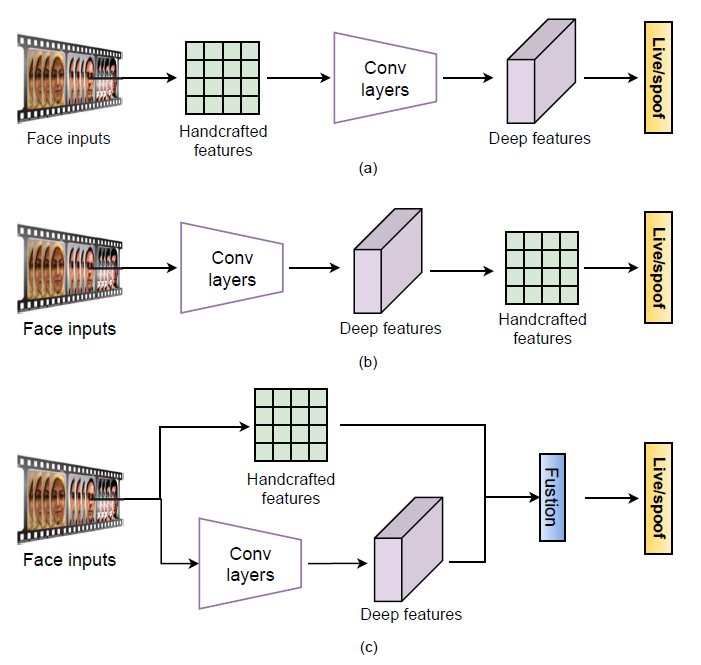
\includegraphics[width=0.5\linewidth]{cnn-hand}}
	\caption{حالت‌های مختلف ترکیب ویژگی‌های دستی و ویژگی‌های یادگیری عمیق \cite{yu2021deep}}
	\label{fig:cnn-hand}
\end{figure}

برای مثال فنگ و همکاران 
\cite{li2016original} 
پیشنهاد داده‌اند که از شبکه‌ی از قبل آموزش داده شده استفاده شود. بدین صورت که از شبکه
 VGG-face \cite{parkhi2015deep}
 که برای تشخیص چهره، روی حجم زیادی داده آموزش داده شده است، استفاده می‌شود و این شبکه روی داده‌های مربوط به کشف تقلب، تنظیم دقیق1 می‌گردد. در مرحله بعد از وزن‌های بهبود یافته استفاده می‌شود و تصاویر نمونه به شبکه داده می‌شود و سپس مقادیر لایه‌های میانی شبکه، به‌صورت ماتریسی روی هم قرار داده می‌شوند و میانگین گرفته می‌شود سپس مقادیری که مقدار زیادی دارند نگه داشته می‌شوند و بعد آن‌ها با الگوریتم PCA کاهش داده می‌شود. سپس ماتریس کاهش بعد داده شده به یک طبقه بند SVM داده می‌شود و تصمیم‌گیری انجام می‌شود. 

لی و همکاران ابتدا یک شبکه عصبی VGG-face را روی داده‌های مربوط به تشخیص تقلب تنظیم دقیق کرده‌اند و سپس روی کانال‌های مختلف در لایه‌های شبکه، عملگر LBP را اعمال کرده‌اند. با گرفتن هیستوگرام روی آن از SVM برای طبقه بندی استفاده کرده‌اند
\cite{li2019face}.
رحمان و همکاران روی تصویر ورودی عملگر LBP زده‌اند و با ترکیب ویژگی‌های لایه اول کانولوشن و خروجی LBP را به ادامه شبکه عصبی داده‌اند
\cite{rehman2020enhancing}. 
 این ایده در شکل
\ref{fig:rahman}
نشان داده شده است.

روش‌های ترکیبی بین ویژگی‌های دستی و ویژگی‌های یادگیری عمیق دارای یک قسمت ایستا هستند که حین آموزش شبکه تغییری نخواهند کرد. برای روش‌های مبتنی بر شبکه عصبی مطلوب این است که تمامی قسمت‌های شبکه به‌صورت انتها به انتها یاد گرفته شود.
\begin{figure}[hb]
	\centerline{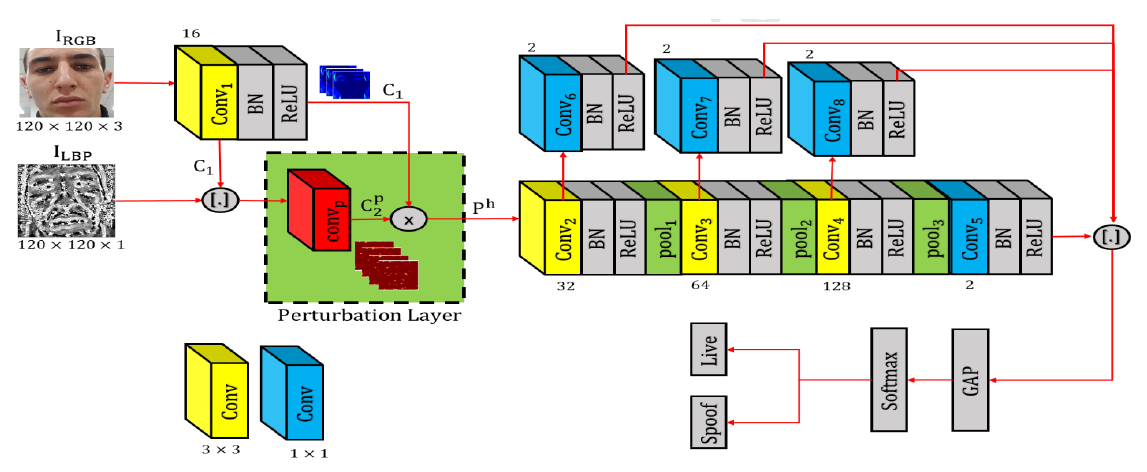
\includegraphics[width=0.5\linewidth]{rahman}}
	\caption{روش ترکیب LBP و کانولوشن \cite{rehman2020enhancing}}
	\label{fig:rahman}
\end{figure}

\subsection{استفاده از تخمین سیگنال کمکی}
در روش‌های بیان شده روال آموزش شبکه عصبی بهینه کردن تابع هزینه آنتروپی متقاطع دودویی1 است. با این رویکرد که در انتهای شبکه یک نورون برای تصمیم‌گیری وجود دارد و تابع هزینه روی این نورون اعمال می‌شود. مشکل این روش این است که شبکه ممکن است ویژگی‌های غیر مطلوبی را پیدا کند که هر چند در جداسازی داده‌های آموزش مفید است اما ممکن است مشابه این ویژگی‌ها در داده‌های آزمون وجود نداشته باشد. این مشکل با عنوان بیش‌برازش2 در علم یادگیری ماشین شناخته می‌شود.

\begin{figure}[h]
	\centerline{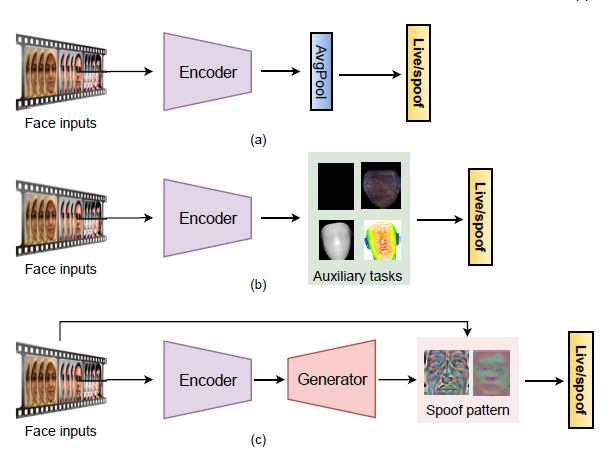
\includegraphics[width=0.7\linewidth]{cnn-aux-methods}}
	\caption{روش‌های مختلف یادگیری عمیق در حوزه‌ی کشف تقلب چهره \cite{yu2021deep}}
	\label{fig:cnn-aux-methods}
\end{figure}

برای مثال ممکن است شبکه در حین آموزش به قاب صفحه نمایشی که برای حمله استفاده شده است توجه کند، اما در داده‌های آزمون مشابه این قاب وجود نداشته باشد. بدین منظور تلاش محققان برای یافتن ویژگی‌های خوش‌ساخت1 به ایده نظارت کمکی2 رسانده است
\cite{liu2018learning}.  
در روش‌های نظارت کمکی سعی می‌شود از تخمین یک مورد کمکی برای استنتاج تقلبی یا واقعی بودن چهره استفاده شود. یکی از موارد مهم کمکی در این حوزه تخمین عمق صورت است.


به‌طور کلی روش دقیق برای محاسبه عمق، استفاده از دوربین مخصوص است که برای هر پیکسل مقدار متناظر با عمق آن پیکسل را نیز بدهد. همچنین با استفاده از روش‌های سه‌بعدی‌سازی و استفاده از حداقل دو دوربین، بازسازی مدل سه‌بعدی امکان پذیر است. اما در کشف تقلب در حالت نرم‌افزاری مطلوب این است که این کار به وسیله‌ی تنها یک دوربین ساده انجام شود. لذا در این حالت تنها می‌توان تخمینی از عمق را داشت.


استفاده از عمق از این شهود گرفته شده است که مغز انسان چهره واقعی را دارای عمق می‌بیند، برای مثال بینی نزدیک‌تر از گونه‌ها است، اما چهره تقلبی که روی صفحه نمایش یا کاغذ چاپ شده قرار دارد دارای عمقی مسطح است. در روش‌هایی که از عمق به‌عنوان یک سیگنال کمکی استفاده کرده‌اند، پیش از آموزش شبکه کشف تقلب، از یک شبکه تخمین عمق مثل 
PRNet \cite{feng2018joint} 
استفاده می‌شود. و عمق به‌دست آمده را بین صفر و یک نرمالایز می‌شود. برای تصاویر واقعی این تصویر به‌عنوان عمق ذخیره شده و برای تصاویر تقلبی، عمق مسطح صفر در نظر گرفته می‌شود. اکنون از این برچسب عمق برای آموزش ساختار شبکه عصبی توسعه داده شده استفاده می‌شود
\cite{atoum2017face,yu2020searching,shao2019multi,liu2018learning,wang2020deep,wang2018exploiting}.
\begin{figure}[h]
	\centerline{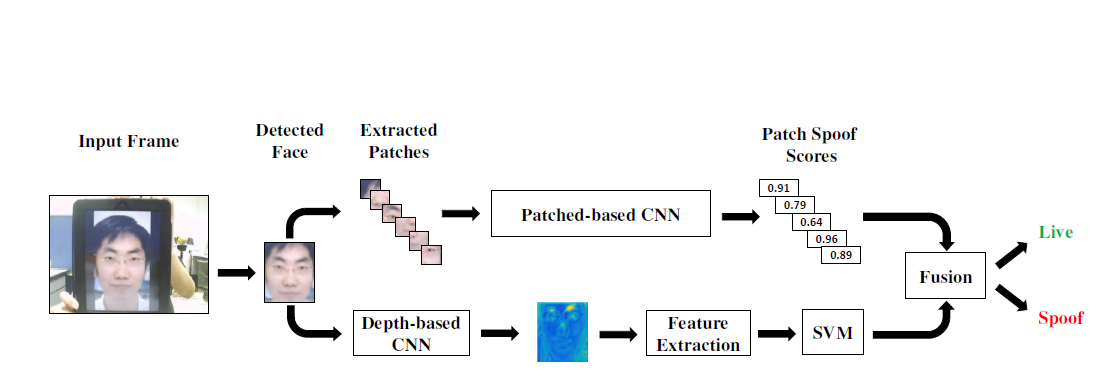
\includegraphics[width=\linewidth]{cnn-depth}}
	\caption{استفاده از عمقب برای کشف تقلب در چهره  \cite{atoum2017face}}
	\label{fig:cnn-depth}
\end{figure}

اتوم و همکاران
\cite{atoum2017face}
  برای اولین بار در این حوزه از عمق به‌عنوان سیگنال کمکی استفاده کرده‌اند. روش ارائه شده بدین صورت است که ابتدا از تصویر ورودی، صورت تشخیص داده شده و تصویر صورت به دو شبکه داده می‌شود. در مسیر بالایی شکل
\ref{fig:cnn-depth}
   قسمت‌های مختلف صورت به‌صورت تصادفی انتخاب شده و به یک شبکه عصبی کانولوشنی داده می‌شود و در مسیر پایین از طریق یک شبکه عصبی، عمق تصویر تخمین زده می‌شود. سپس اطلاعات دو مسیر با یکدیگر ترکیب شده و در مورد واقعی یا غیرواقعی بودن تصویر تصمیم‌گیری می‌شود.
   
   همچنین لیو و همکاران
\cite{liu2018learning}
   علاوه بر استفاده از سیگنال کمکی عمق از تخمین سیگنال rPPG در طول فریم‌های متوالی به‌عنوان سیگنال حیات چهره بهره برده‌اند. در قسمت عمق مشابه
\cite{atoum2017face}
   ابتدا برچسب عمق واقعی برای چهره زنده و عمق صفر برای چهره تقلبی تخمین زده شده و از تابع هزینه رابطه
\ref{eq:depthreg}
   برای بهینه سازی شبکه استفاده می‌شود. که در آن  عمق متناظر با تصویر  است.
\begin{equation}\label{eq:depthreg}
	\Theta_D = \argmin_\Theta{\sum_{i=1}^{N_d}||CNN_D(I_i;\Theta)-D_i||^2_1} 
\end{equation}

\begin{figure}[t]
	\centerline{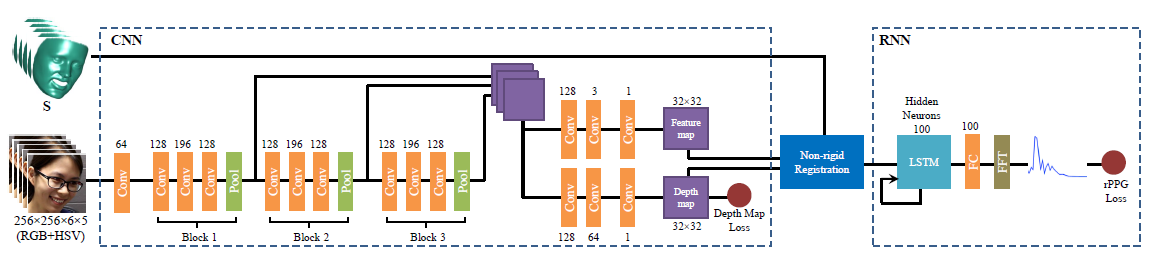
\includegraphics[width=\linewidth]{depth-rppg}}
	\caption{روش استفاده از عمق و تخمین rPPG \cite{liu2018learning}}
	\label{fig:depth-rppg}
\end{figure}

همچنین ونگ و همکاران
\cite{wang2018exploiting}
ساختاری را به کمک optical flow روی ویژگی‌های شبکه عصبی برای تخمین عمق توسعه داده‌اند، به‌گونه‌ای که اطلاعات حرکتی بین فریم‌های متوالی نیز در نظر گرفته می‌شود. همچنین از ترکیب ساختار
 GRU \cite{cho2014learning}
با کانولوشن بلوکی به نام ConvGRU معرفی کرده‌اند که در آن در رابطه GRU به‌جای ضرب‌های ماتریسی از عملگر کانولوشن استفاده شده است و کاربرد آن توجه به ویژگی‌های بلند مدت در میان فریم‌های متوالی ورودی است.

\begin{figure}[h]
	\centerline{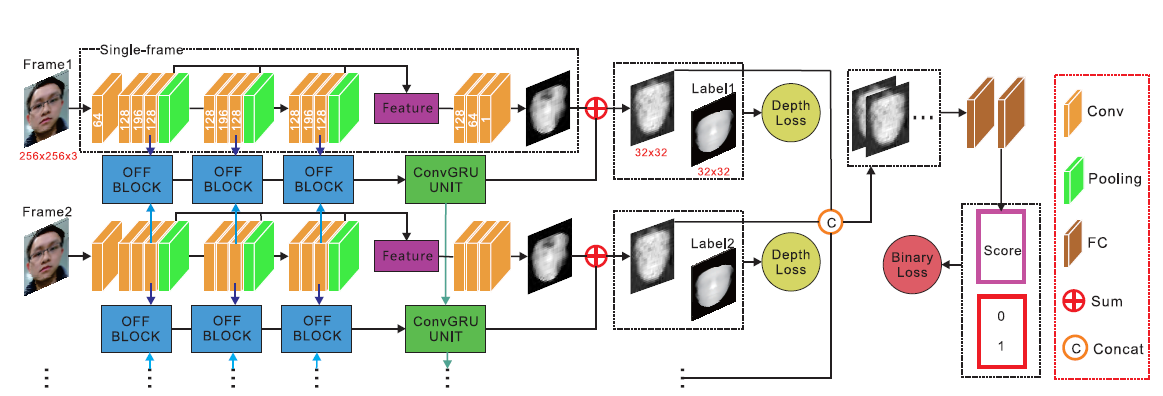
\includegraphics[width=\linewidth]{wang}}
	\caption{استفاده از ویژگی‌های عمیق در طول زمان \cite{wang2018exploiting}}
	\label{fig:wang}
\end{figure}
در استفاده از سیگنال کمکی عمق در شبکه نه تنها مقدار عمق می‌تواند مهم باشد بلکه پیوستگی عمق بین پیکسل‌های مجاور نیز اهمیت دارد. بدین منظور تابع هزینه CDL برای در نظر گرفتن این پیوستگی عمق در پیکسل‌های مجاور توسعه داده شده است
\cite{wang2020deep,wang2018exploiting}
در تابع هزینه CDL به‌جای محاسبه فاصله اقلیدسی عمق تخمینی و برچسب عمق به‌صورت پیکسل به پیکسل مشابه رابطه
\ref{eq:cdl}
، از تفاوت عمق بین پیکسل‌های مجاور نیز استفاده می‌شود.
\begin{equation}\label{eq:cdl}
	L_{CDL} = \sum_{i}||K_i^{CDL} \odot D_P-K_i^{CDL} \odot D_G||
\end{equation}
که در آن
$D_P$
عمق تخمین زده شده توسط شبکه و
$D_G$
عمق برچسب واقعی است و
$K_i^{CDL}$
هسته‌های کانولوشن دارای 0 و 1 و-1 هستند که در شکل
\ref{fig:cdl}
نشان داده شده است. و  نشانگر عملگر کانولوشن است. در شکل
\ref{fig:cdl}
مربع بنفش متناظر با عدد 1- و مربع زرد متناظر با عدد 1 و مربع‌های سفید عدد 0 را در هسته نشان می‌دهند. 
 \begin{figure}[ht]
 	\centerline{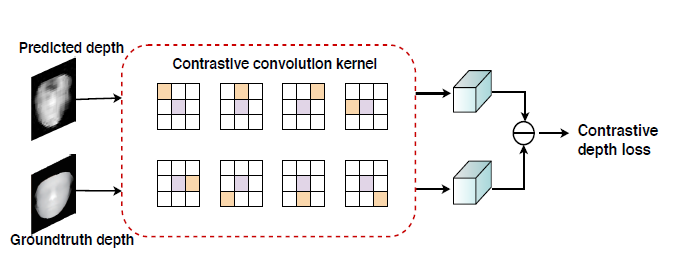
\includegraphics[width=0.5\linewidth]{cdl}}
 	\caption{نحوه محاسبه تابع هزینه CDL}
 	\label{fig:cdl}
 \end{figure}
یو و همکاران
\cite{yu2020searching}
ساختاری تغییر یافته از شبکه‌های کانولوشنی با تأکید بر پیکسل مرکزی پنجره کانولوشن توسعه داده‌اند که درشکل
\ref{fig:central-dif}
نشان داده شده است.
این ساختار با الهام از LBP ایجاد شده است، به‌گونه‌ای که در هر بار انجام عملگر کانولوشن، پیکسل مرکزی از پیکسل‌های مجاور کم خواهد شد. که رابطه
\ref{eq:central-dif1}
این عملگر را نشان می‌دهد.
\begin{equation}\label{eq:central-dif1}
	y(p_0) = \sum_{p \in R} w(p_n).(x(p_0+p_n)-x(p_0)) 
\end{equation}
برای آنکه از خاصیت کانولوشن نیز استفاده شود ترکیب خطی رابطه
\ref{eq:central-dif1}
با رابطه کانولوشن حساب می‌گردد.
\begin{equation}\label{eq:central-dif2}
	y(p_0) = \theta\sum_{p \in R} w(p_n).(x(p_0+p_n)-x(p_0)) +
	(1-\theta)\sum_{p \in R}w(p_n).(x(p_0+p_n)
\end{equation}
که در آن
$\theta$
یک هایپر پارامتر است و قسمت اول رابطه
\ref{eq:central-dif2}
کانولوشن تفاضلی مرکزی و قسمت دوم کانولوشن کلاسیک است. این رابطه در نهایت به‌صورت رابطه
\ref{eq:central-dif3}
ساده می‌گردد.
\begin{equation}\label{eq:central-dif3}
	y(p_0) = \sum_{p \in R} {w(p_n).x(p_0+p_n)} +
	\theta(-x(p_0)\sum_{p \in R}{w(p_n)}
\end{equation}
\begin{figure}[h]
	\centerline{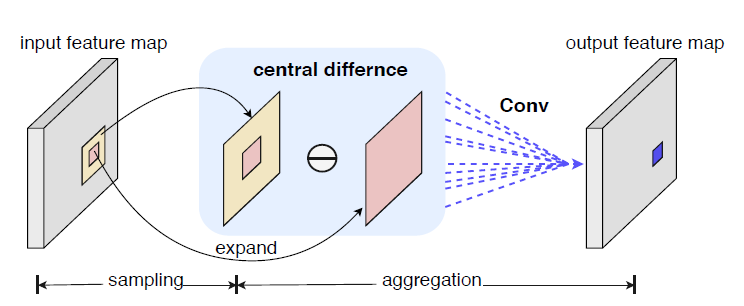
\includegraphics[width=0.5\linewidth]{central-dif}}
	\caption{عملگر کانولوشن تغییر یافته \cite{yu2020searching} }
	\label{fig:central-dif}
\end{figure}

که همانطور که مشاهده می‌شود که همان کانولوشن کلاسیک خواهد بود که پیکسل مرکزی وزن متفاوتی نسب به کانولوشن کلاسیک خواهد داشت. از این ساختار برای تخمین سیگنال کمکی عمق با نظارت تابع هزینه CDL کمک استفاده می‌شود. همچنین برای یافتن اندازه‌ی شبکه از روش جستجوی معماری شبکه1 
\cite{zoph2016neural}
استفاده شده است.

در جستجوی معماری شبکه بر خلاف روش‌های کلاسیک که طراحی معماری شبکه با مهندسی و سعی و خطا انجام می‌شود، تلاش می‌شود معماری بهینه برای کاربرد مورد نظر به‌صورت خودکار با یادگیری تقویتی و مفاهیم یادگیری ماشین پیدا شود. در حوزه کشف تقلب علاوه بر
\cite{zoph2016neural}
کارهای
\cite{yu2020fas,yu2020auto} 
متدهایی بر پایه این ابزار برای یافتن شبکه بهینه پیشنهاد داده‌اند.
 
 لی و همکاران به‌جای تخمین عمق در یک صفحه دو بعدی، از ابر نقاط در فضای سه‌بعدی به‌عنوان سیگنال کمکی استفاده کرده‌اند و ساختاری به نام 3DPC-NET پیشنهاد کرده‌اند
\cite{li20203dpc}.
 
 یو و همکاران 
\cite{yu2020face}
 مسئله تشخیص تقلب در چهره را یک مسئله تشخیص ماده فرض کرده‌اند. این فرض با توجه به این واقعیت استفاده شده است که جنس پوست صورت با جنس کاغذ چاپ‌شده و جنس صفحه‌ی نمایش متفاوت است. برای تشخیص جنس ماده با الهام از فیلتر bilateral روی ویژگی‌های شبکه عمیق از این فیلتر استفاده کرده‌اند. فیلتر bilateral میانگین وزن‌دار روی پیکسل‌های مجاور است که با افزایش فاصله تأثیر آن به‌صورتی تابعی گوسی کاسته می‌شود و روی هر پیکسل به مختصات p و تصویر I به‌صورت رابطه 
\ref{eq:bilat}  
 تعریف می‌شود.
\begin{equation}\label{eq:bilat}
	BiBase(I_p)=\frac{1}{k}\sum_{q\in I}{g_{\sigma_s}(||p-q||)g_{\sigma_r}(||I_p-I_q||)I_q}
\end{equation}
\begin{equation}\label{eq:bilat}
	k=\sum_{q\in I}{g_{\sigma_s}(||p-q||)g_{\sigma_r}(||I_p-I_q||)}
	\nonumber
\end{equation}

که در آن
$g_\sigma (x) = \exp(\frac{-x^2}{\sigma^2})$
تابع گوسی است. در این روش ساختار شبکه مشابه
\cite{liu2018learning}
 است ولی روی ویژگی‌های کانولوشن این فیلتر اعمال شده است.
 
\begin{figure}[t]
 	\centerline{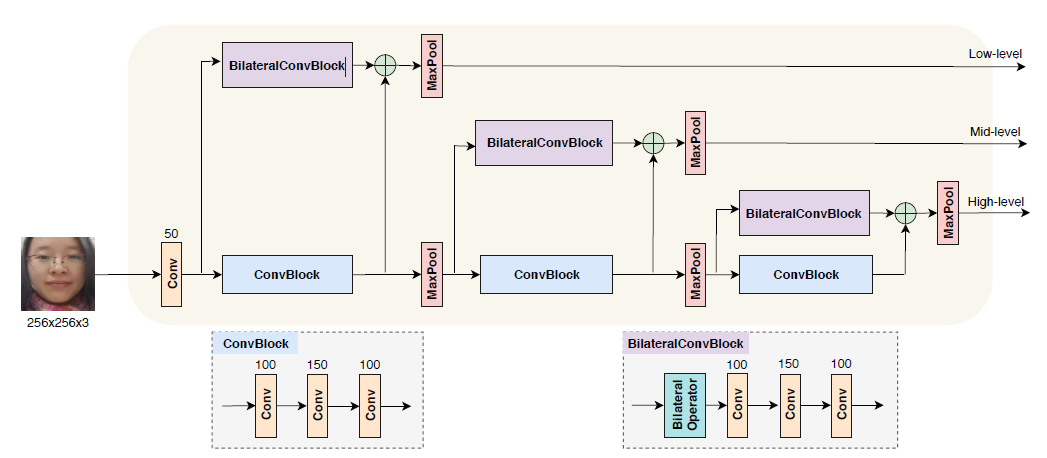
\includegraphics[width=0.7\linewidth]{bilat}}
 	\caption{روش استفاده از فیلتر bilateral در شبکه عمیق \cite{yu2020face} }
 	\label{fig:bilat}
\end{figure}

با وجود آن‌که سیگنال کمکی عمق در ادبیات موضوع به‌طور گسترده استفاده شده است اما پر هزینه است و نیاز به پردازش بیشتر برای تخمین عمق دارد. جدای از آن‌که عمق، یک سیگنال کامل برای تشخیص تقلب نیست و فرض مسطح در نظر گرفتن عمق در چهره‌های تقلبی، فرض همیشه برقرار نیست. برای مثال فرض کنید مهاجم ابزار حمله مثل صفحه نمایش یا کاغذ چاپ شده را به‌صورت مایل قرار دهد در این صورت عمق به‌صورت یکنواخت در همه‌جا صفر نخواهد بود.

 جرج و مارسل روشی را برای پیدا کردن ویژگی‌های خوش‌ساخت بدون استفاده از عمق پیشنهاد کرده‌اند
 \cite{george2019deep}.
 در این روش از چند لایه اول شبکه DENSNET
\cite{huang2017densely}
برای نشان‌کردن تصویر ورودی به یک صفحه 14*14 استفاده کرده‌اند. و قرارداد کرده‌اند که برچسب واقعی به‌جای یک عدد صفر و یک، یک ماتریس دو بعدی به طول کامل صفر یا یک است و تابع هزینه آنتروپی متقاطع دودویی را به‌جای یک نورون روی یک صفحه دو بعدی در نظر گرفته‌اند. با این روش دیگر نیازی به تخمین عمق نخواهد بود.
\begin{figure}[h]
	\centerline{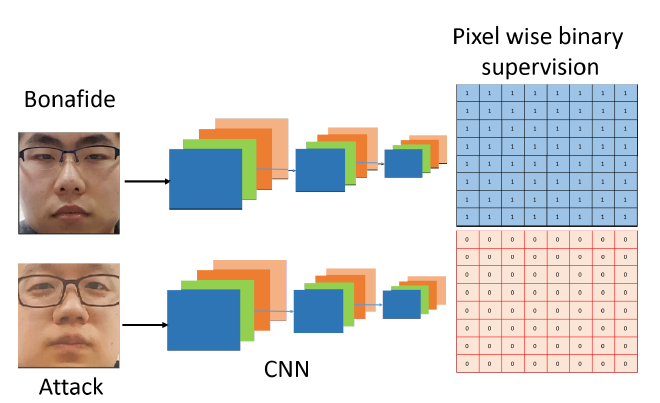
\includegraphics[width=0.5\linewidth]{pixel-wise}}
	\caption{تابع هزینه BCE روی یک صفحه مسطح به‌جای یک نورون \cite{george2019deep} }
	\label{fig:pixel-wise}
\end{figure}
\subsection{استفاده از شبکه‌های مولد تهاجمی و تابع هزینه‌های مختلف}
مسئله کشف تقلب در تشخیص چهره بیشتر شبیه مسئله یافتن یک نویز خاص در تصویر است. ابزارهای حمله نظیر کاغذ چاپ‌شده و صفحه نمایش‌گر، بافت و تفکیک‌پذیری متفاوتی با بافت صورت انسان دارند. که این تفاوت جنس را می‌توان با یک نویز جمع شونده با تصویر چهره انسان زنده مدل کرد. جورابلو و همکاران
\cite{jourabloo2018face}
برای اولین بار مسئله کشف تقلب در چهره از شبکه‌های مولد تهاجمی1 (GAN)
\cite{goodfellow2014generative}
رای مدل کردن و یافتن نویز تصاویر تقلبی استفاده کرده‌اند. با تخمین نویز مربوط به کشف تقلب، قدرت استنتاج برای تقلبی بودن تصویر بیشتر خواهد شد.

از آنجا که نویز مربوط به تقلب می‌تواند در سطوح مختلف در تصویر وجود داشته باشد لیو و همکاران
\cite{liu2020disentangling}
ساختاری بر پایه GAN که الگوهای تقلب در ابعاد مختلف تصویر را تخمین بزند پیشنهاد داده‌اند. در این روش در شبکه مولد dismantlement generator ابعاد تصویر در لایه‌های اول کاهش یافته و سپس افزایش می‌یابد و از ویژگی‌های خروجی لایه‌ها با ابعاد مختلف به‌عنوان ویژگی‌های تقلب تولید شده استفاده می‌شود. در نهایت شبکه multiscale discriminator این ویژگی‌های تقلب در سطوح مختلف را به‌عنوان ورودی دریافت می‌کند و طی یک بازی رقابتی بین دو شبکه در GAN در نهایت ویژگی‌های تقلب بهتری تولید خواهد شد. 
\begin{figure}[h]
	\centerline{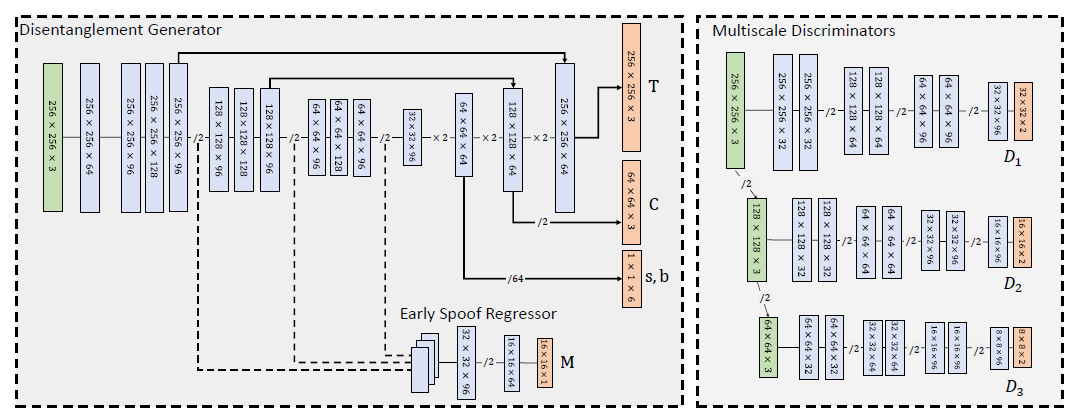
\includegraphics[width=0.7\linewidth]{distang}}
	\caption{ساختار بر پایه استفاده از شبکه مولد برای تخمین علائم تقلب در سطوح مختلف \cite{liu2020disentangling} }
	\label{fig:pixel-wise}
\end{figure}

با وجود اینکه در دو پژوهش اخیر ذکر شده
\cite{jourabloo2018face,liu2020disentangling}
از شبکه مولد تهاجمی برای بهبود دقت در تست درون دیتاست استفاده شده است، توجه پژوهشگران به استفاده از GAN برای تعمیم‌پذیری مدل در دیتاست‌های مختلف جلب شده است
\cite{shao2019multi,jia2020single}.

تعمیم‌پذیری مدل در دیتاست‌های مختلف بدین معناست که برای مثال از بین چهار دیتاست مختلف، سه دیتاست برای آموزش شبکه استفاده می‌گردد و مدل آموزش داده شده روی دیتاست چهارم آزمایش می‌شود. از آنجا که دیتاست‌های مختلف توزیع‌های متفاوتی دارند، رسیدن به دقت خوب در تست روی دیتاست دیده نشده (که توزیع لزوماً یکسانی با توزیع دیتاست‌هایی که برای آموزش استفاده شده است ندارد) یک چالش جدی در این حوزه است. 

همچنین یک روش برای بهبود قابلیت تعمیم‌پذیری، استفاده از تابع هزینه سه‌گانه1 
\cite{schroff2015facenet}
است. در تابع هزینه سه‌گانه هدف این است که استخراج ویژگی به نحوی انجام شود که فاصله ویژگی‌های نمونه‌های مربوط به یک کلاس کوچک و فاصله بین نمونه‌های مربوط به کلاس‌های مختلف زیاد شود.

فرض کنید خروجی شبکه استخراج ویژگی بردار  باشد. در این صورت برای تشکیل تابع هزینه سه‌گانه لازم است که از خروجی‌های شبکه استخراج ویژگی، یک بردار ویژگی لنگر ، یک بردار ویژگی با برچسب یکسان با لنگر  و یک بردار ویژگی با برچسب متفاوت با لنگر   انتخاب شود. تابع هزینه سه گانه به‌صورت رابطه
\ref{eq::tripl}
 تعریف می‌شود.که در آن  یک حاشیه از قبل تعریف شده است. تمام سه‌گانه‌هایی که فاصله درون کلاسی آن‌ها از فاصله برون کلاسی بیشتر از مقدار  است درون مجموع گیری قرار می‌گیرد.که در آن  یک حاشیه از قبل تعریف شده است. تمام سه‌گانه‌هایی که فاصله درون کلاسی آن‌ها از فاصله برون کلاسی بیشتر از مقدار  است درون مجموع گیری قرار می‌گیرد.
 
 \begin{equation}\label{eq:tripl}
L_{trpi} = \sum_{i}{[||f(x_i^a)-f(x_i^p)||_2^2-||f(x_i^a)-f(x_i^n)||_2^2+\alpha]_+}
 \end{equation}

تابع هزینه سه‌گانه به‌صورت رابطه
\ref{eq:tripl1}
نیز قابل بیان است.که در آن زمانی که فاصله درون کلاسی کوچکتر از فاصله برون کلاسی به میزان سطح آستانه  باشد حاصل max صفر خواهد بود و در محاسبات تابع هزینه نقش نخواهد داشت.
 \begin{equation}\label{eq:tripl1}
	L_{trpi} = \sum_{i}{max(0,||f(x_i^a)-f(x_i^p)||_2^2-||f(x_i^a)-f(x_i^n)||_2^2+\alpha)}
\end{equation}

\begin{figure}[t]
	\centerline{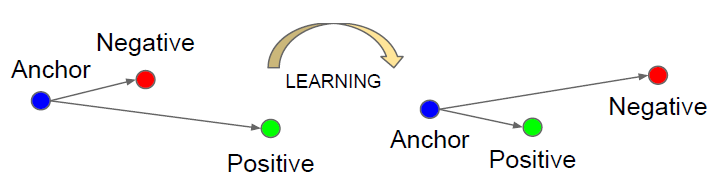
\includegraphics[width=0.7\linewidth]{trip}}
	\caption{نحوه عملکرد تابع هزینه سه‌گانه روی فاصله بردارهای ویژگی \cite{schroff2015facenet} }
	\label{fig:trip}
\end{figure}
شائو و همکاران
\cite{shao2019multi}
از ساختار GAN و ابزار کمکی تخمین عمق و تابع هزینه سه‌گانه برای بهبود تعمیم‌پذیری استفاده کرده‌اند. در این کار یک تابع هزینه بر مبنای تابع هزینه‌ی سه‌گانه توسعه داده شده است که فاصله بین نمونه‌ها با برچسب یکسان در دیتاست‌های مختلف را کوچک‌تر کند و فاصله نمونه‌ها با برچسب متفاوت در یک دیتاست را بیش‌تر کند. با این‌کار توزیع نمونه‌ها در دیتاست‌های مختلف با یک‌دیگر متراکم‌تر خواهد شد. در شکل
\ref{asym} 
به‌کارگیری این تابع هزینه را در بین دو دیتاست مختلف نشان می‌دهد.

\begin{figure}[h]
	\centerline{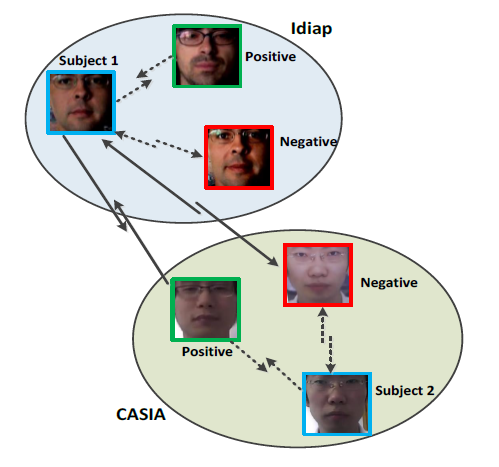
\includegraphics[width=0.4\linewidth]{asym}}
	\caption{نحوه اثر تابع هزینه روی فاصله نمونه‌ها در دیتاست‌های مختلف \cite{shao2019multi} }
	\label{fig:asym}
\end{figure}

همچنین جیا و همکاران
\cite{jia2020single}
 علاوه بر استفاده از GAN صورتی نامتقارنی از تابع هزینه سه‌گانه را پیشنهاد کرده‌اند. به‌گونه‌ای که نمونه‌های زنده در دیتاست‌های مختلف به یک‌دیگر نزدیک‌تر شوند و نمونه‌های تقلبی در دیتاست‌های مختلف از یک دیگر دورتر شده و نمونه‌های واقعی از نمونه‌های تقلبی با فاصله باشند. 
 
 \begin{figure}[h]
 	\centerline{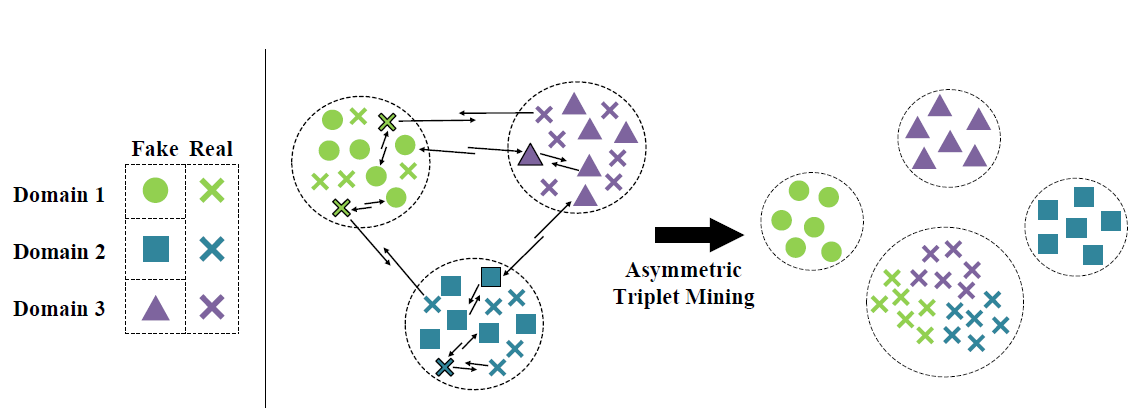
\includegraphics[width=\linewidth]{jia}}
 	\caption{تابع هزینه نامتقارن برای کاهش فاصله نمونه‌های از یک کلاس \cite{jia2020single} }
 	\label{fig:jia}
 \end{figure}

فنگ و همکاران
\cite{feng2020learning}
یک ساختار U-Net
\cite{ronneberger2015u}
به کار برده‌اند و در میان لایه‌های آخر شبکه تولید کننده الگوهای تقلب از تابع هزینه سه‌گانه استفاده کرده‌اند و خروجی این شبکه U-Net را به یک شبکه طبقه بند کمکی داده‌اند.

 \begin{figure}[h]
	\centerline{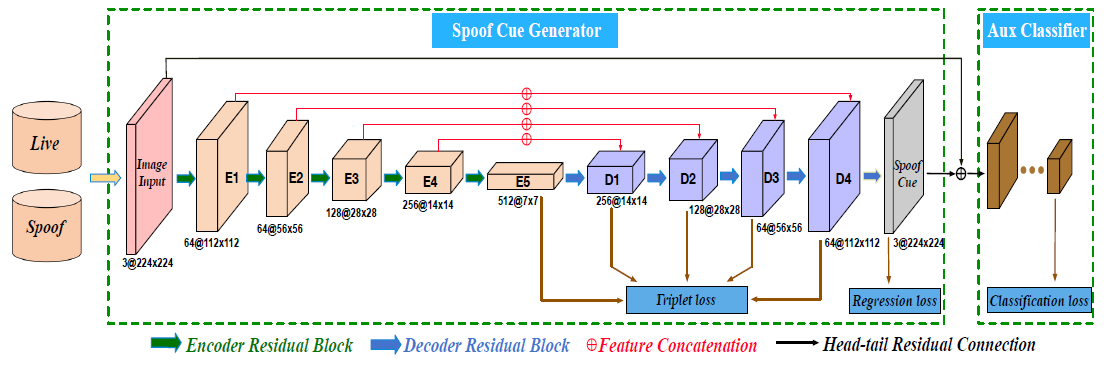
\includegraphics[width=\linewidth]{cue}}
	\caption{ساختار U-net و تابع هزینه سه‌گانه \cite{feng2020learning} }
	\label{fig:cue}
\end{figure}

پرزکابو و همکاران
\cite{perez2019deep}
ابع هزینه سه‌گانه را در فضای نمایی به کار برده‌اند که در رابطه
\ref{eq:ltf}
نشان داده شده است.
 \begin{equation}\label{eq:ltf}
	L_{tf} = \sum_{i}{max(0,e^{\frac{D_{a,p}}{\sigma}}-e^{\frac{D_{a,n}}{\sigma}}+\alpha)}
\end{equation}

که در آن
$D_{a,p}$
فاصله درون‌کلاسی و
$D_{a,n}$
فاصله برون‌کلاسی است و
$\sigma$
یک هایپر پارامتر است.

جرج و مارسل
\cite{george2020learning} 
 تابع هزینه‌ای معرفی کرده‌اند که در فضای n بعدی بردارهای ویژگی، نمونه‌های زنده نزدیک به یک مرکز قرار بگیرند و نمونه‌های تقلبی با یک حاشیه از این مرکز فاصله داشته باشند. مرکز نمونه‌های واقعی در حین آموزش شبکه به‌روزرسانی می‌شود.
فرض کنید مرکز نمونه‌های زنده با  نشان داده شود و فاصله بردار ویژگی نمونه i با مرکز با  تعریف شود. در این صورت تابع هزینه تعریف شده به‌صورت رابطه
\ref{eq:occl}
است.
 \begin{equation}\label{eq:occl}
L_{OCCL}=Y\frac{1}{2}DC^2_W+(1-Y)\frac{1}{2}\max(0,m-DC_W)^2
\end{equation}
که در آن Y برچسب واقعی داده است که برابر با یک است اگر نمونه واقعی باشد و صفر است اگر نمونه تقلبی باشد و m یک حاشیه از قبل تعریف شده است.
 \begin{figure}[h]
	\centerline{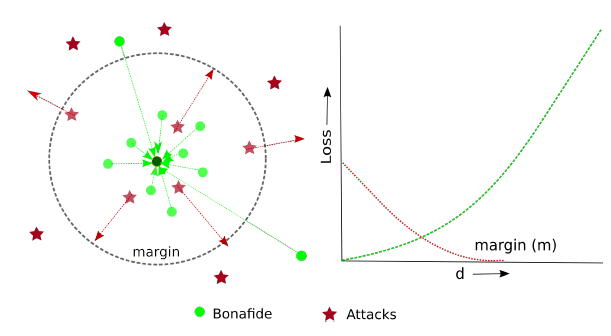
\includegraphics[width=0.5\linewidth]{geo}}
	\caption{کاهش فاصله نمونه‌های واقعی تا مرکز و افزایش فاصله نمونه‌های تقلبی تا مرکز \cite{george2020learning} }
	\label{fig:geo}
\end{figure}

تو و همکاران
\cite{tu2020learning}
 نیز شبکه VGG-face را به‌صورت همزمان با دو هدف شناسایی چهره و تشخیص تقلب آموزش داده‌اند و یک تابع هزینه معرفی کرده‌اند که هدف آن منظم‌سازی1 و جلوگیری از بیش برازش شبکه است. در این تابع فاصله بین هر دو جفت نمونه داده‌ها مستقل از آنکه برچسب آنچه باشد کاهش داده می‌شود. تابع هزینه معرفی شده برای این هدف در رابطه
\ref{eq:tpc}
 بیان شده است. که در آن تابع 
 $\Phi(.)$
  نشان دهنده رابطه بین ورودی تصویر و لایه یکی به آخر شبکه است و M تمام جفت نمونه‌های موجود در دسته آموزش است. 
  \begin{equation}\label{eq:tpc}
 	L_{tpc}=\sum_{i\ne j}^{M}||\Phi(x_i)-\Phi(x_j)||
 \end{equation}

ژنگ و همکاران
\cite{zhang2020face}
علاوه بر تخمین عمق از تخمین LBP به‌عنوان سیگنال کمکی استفاده کرده‌اند که در کنار عمق ساختار LBP تصویر ورودی نیز تخمین زده‌شود. بدین ترتیب که برای تصاویر تقلبی خروجی LBP شبکه باید صفر باشد و برای تصاویر تصاویر واقعی خروجی قسمت LBP باید معادل LBP تصویر ورودی باشد. این شبکه دارای یک شبکه مولد با ساختار U-net و سه شبکه طبقه‌بند برای عمق و LBP و شبکه طبقه بندی بر اساس GAN برای تصویر واقعی و ساختگی است.
 \begin{figure}[h]
	\centerline{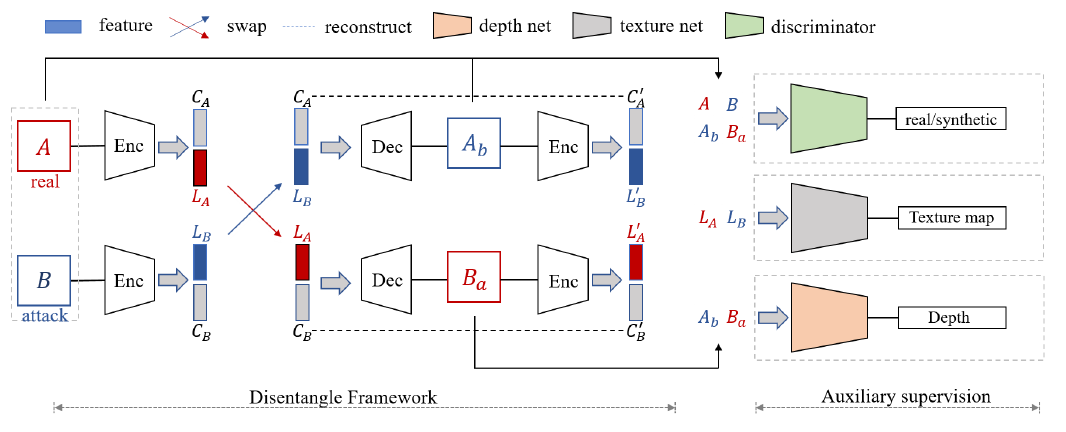
\includegraphics[width=0.7\linewidth]{zhang}}
	\caption{استفاده از LBP در کنار عمق برای یافتن ویژگی‌های خوش ساخت \cite{zhang2020face} }
	\label{fig:zhang}
\end{figure}

ژو و همکاران
\cite{xu2021improving}
روی ثبات فضای ویژگی در بین فریم‌های متوالی یک ویدئو تأکید کرده‌اند. در این کار به‌جای استفاده از الگوریتم‌های تشخیص چهره در هر فریم از الگوریتم دنبال‌کننده‌ی چهره استفاده کرده و چهره‌های تخمین زده شده در فریم‌های متوالی را به شبکه تشخیص تقلب داده‌اند. برای این شبکه تابع هزینه‌ای ارائه معرفی کرده‌اند که فاصله بین بردارهای ویژگی یک ویدئو در دیتاست را کوچک‌تر کند. 
  \begin{equation}\label{eq:xult}
	L_{t}=\frac{1}{m}\sum_{i=0}^{m}\max_{i,j \in v}{||x_i-x_j||^2}
\end{equation}
که در آن m اندازه دسته آموزش است و
$x_i,x_j$
بردارهای فضای ویژگی برای یک ویدئو است. همچنین برای ثبات بردارهای ویژگی در ویدیوهای مختلف، تابع هزینه‌ی دیگری پیشنهاد کرده‌اند که فاصله بین بردارهای ویژگی متعلق به یک برچسب واقعی را نیز کوچک‌تر کند.

  \begin{equation}\label{eq:xule}
	L_{t}=\frac{1}{m}\sum_{i=0}^{m}\max{y_{ij}||x_i-x_j||^2}
\end{equation}

که در آن 
$y_{ij}$
  زمانی که دو بردار ویژگی متعلق به یک کلاس باشند برابر با صفر خواهد بود و در غیر این‌صورت صفر است.
  \section{دیتاست‌های مورد استفاده}
  مانند بسیاری از مسائل بینایی ماشین، دیتاست نقش حیاتی در توسعه الگوریتم و سنجش میزان دقت الگوریتم ایفا می‌کند. از آنجا که تمرکز این پایان‌نامه روی حملات کاغذ چاپ‌شده و بازپخش صفحه نمایش است، به معرفی دیتاست‌هایی که حاوی این نوع حملات هستند پرداخته می‌شود. حملات نظیر استفاده از ماسک، معمولاً براحتی قابل اجرا نیستند و هزینه‌بر هستند اما دو حمله گفته شده از نظر قابلیت اجرا ساده‌تر، کم هزینه و متداول‌تر هستند. 
\subsection{دیتاست Replay}
دیتاست Replay شامل ویدیوهای از 50 شخص مختلف با نمونه‌های واقعی و تقلبی است
\cite{chingovska2012effectiveness}
 نمونه‌های واقعی در شرایط محیطی نوری کنترل‌شده با پس‌زمینه یکنواخت و شرایط محیطی با نور کنترل نشده با پس زمینه غیر یکنواخت گرفته شده‌اند. برای نمونه‌های تقلبی از صفحه کاغذ چاپ‌شده، استفاده از تلفن همراه برای بازپخش ویدئو، و استفاده از تبلت iPAD برای پخش ویدئو با کیفیت بالا استفاده شده است. همچنین نمونه‌های تقلبی در دو حالت استفاده از یک پایه ثابت به‌منظور ثابت ماندن ابزار حمله و استفاده از دست که کمی لغزش خواهد داشت گرفته شده‌اند. رزولوشن تمامی نمونه‌ها واقعی و تقلبی با فرمت QVGA یعنی 320*240 پیکسل است.
\begin{figure}[h]
 	\centerline{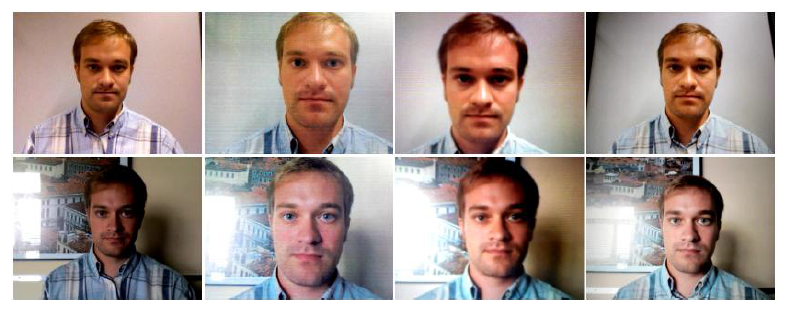
\includegraphics[width=\linewidth]{replay}}
 	\caption{نمونه‌هایی از دیتاست Replay \cite{chingovska2012effectiveness} }
 	\label{fig:replay}
\end{figure}
در
\ref{fig:replay}
نمونه‌هایی از این دیتاست نشان داده شده است. در سطر بالایی نمونه‌ها در محیط کنترل شده از نظر نورپردازی و پس‌زمینه یکنواخت هستند، در حالی که تصاویر سطر پایینی نمونه‌ها دارای نورپردازی غیر کنترل‌شده و پس زمینه غیر یکنواخت هستند. تصاویر از سمت چپ به‌ترتیب تصاویر واقعی، استفاده از کاغذ چاپ‌شده، استفاده از تلفن همراه برای بازپخش و استفاده از تبلت برای بازپخش ویدئو هستند.
\subsection{دیتاست CASIA}
در دیتاست CASIA نیز از 50 شخص مختلف نمونه‌های واقعی و تقلبی گرفته شده است 
\cite{zhang2012face}
. همچنین تصویربرداری با سه نوع دوربین مختلف برای پوشش دادن حالت‌های مختلف در رزولوشن‌های مختلف انجام شده است. در این دیتاست حملات نوع کاغذ چاپ‌شده روی کاغذ گلاسه صورت گرفته است که کیفیت بالاتری نسبت به کاغذ معمولی دارد. همچنین برای حمله بازپخش از تبلت استفاده شده است. در نمونه‌های واقعی دیتاست از کاربر خواسته شده است که پلک و لب بزند تا ویدیوهای ضبط شده دارای اطلاعات حرکتی صورت باشند. در نمونه حمله‌های تقلبی قسمت چشم‌های صورت بریده شده است تا کاربر با پلک زدن بتواند در نمونه‌های تقلبی اطلاعات حرکت به ویدئو بدهد. همچنین در نمونه‌هایی که کاغذ بریده نشده است از کاربر خواسته شده که با حرکت دست کاغذ چاپ شده را حرکت بدهد. نمونه‌هایی از دیتاست CASIA در شکل 
\ref{fig:casia}
نشان داده شده است.

 \begin{figure}[h]
	\centerline{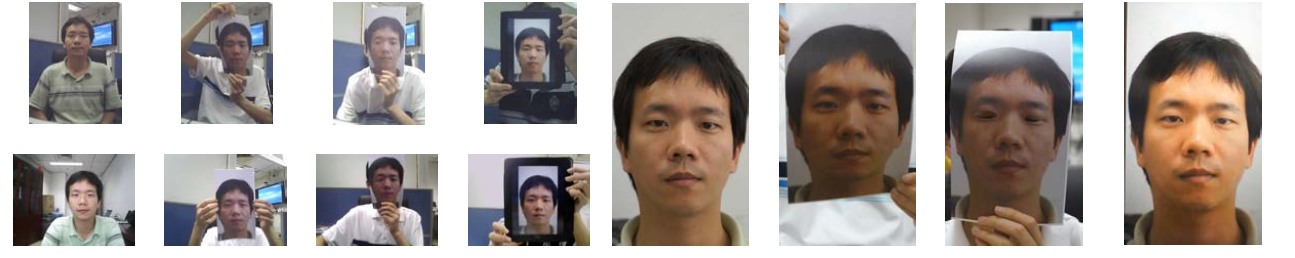
\includegraphics[width=\linewidth]{casia}}
	\caption{نمونه‌هایی از دیتاست CASIA \cite{zhang2012face} }
	\label{fig:casia}
\end{figure}

\subsection{دیتاست MSU}
در دیتاست MSU
\cite{wen2015face}
 از 55 شخص تصویربرداری شده است که ویدیوهای متعلق به 35 فرد در دسترس قرار داده شده است. برای تصویربرداری از دوربین لپ‌تاپ و دوربین تلفن همراه استفاده شده است که دارای رزولوشن 480*640 و 720*480 هستند. استفاده از این نوع دوربین‌ها به‌منظور شبیه‌سازی سناریو احراز هویت از طریق تلفن همراه و لپ‌تاپ انجام شده است. برای حمله باز پخش از صفحه نمایش تبلت و تلفن همراه استفاده شده است. همچنین برای حمله کاغذ چاپ شده از پرینتر با کیفیت استفاده شده است.

 \begin{figure}[h]
	\centerline{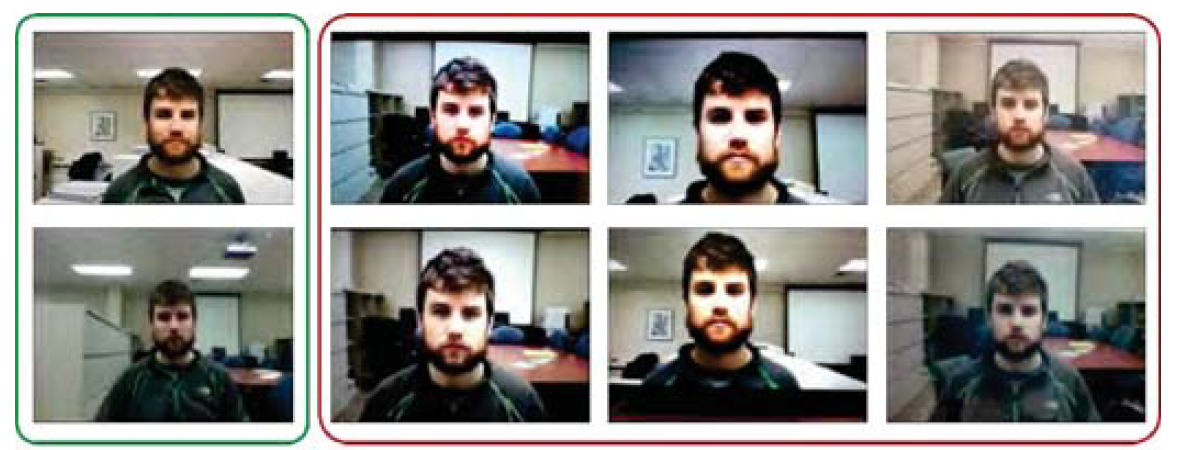
\includegraphics[width=\linewidth]{msu}}
	\caption{نمونه‌هایی از دیتاست MSU \cite{wen2015face} }
	\label{fig:msu}
\end{figure}

\subsection{دیتاست OULU}
در دیتاست OULU
\cite{boulkenafet2017oulu}
از 55 شخص مختلف برای تصویر برداری نمونه‌های واقعی و تقلبی استفاده شده است. تصویربرداری در سه نشست مختلف، با شش تلفن همراه جدید در زمان جمع‌آوری دیتاست استفاده شده است که باعث تنوع در کیفیت تصویر و محیط پس‌زمینه شده است. برای حمله کاغذ چاپ شده از دو نوع چاپگر با کیفیت و برای حمله بازپخش از یک نمایش‌گر و صفحه نمایش لپ‌تاپ استفاده است. ویدیوهای ضبط شده با کیفیت full HD با رزولوشن 1920*1080 گرفته شده است.

این دیتاست در مقایسه با دیتاست‌های قبلی تنوع بیشتر و کیفیت بالاتری دارد که باعث چالشی شدن دیتاست شده‌است. نمونه‌های واقعی در دیتاست OULU در شکل 
\ref{fig:oulureal}
 نشان داده شده است و نمونه‌های حمله در شکل 
 \ref{fig:oulufake}
 نشان داده شده است که دو نمونه‌ی سمت چپ دو نوع حمله کاغذ چاپ‌شده و نمونه‌های سمت راست دو نوع حمله باز پخش را نشان می‌دهد. 
 
  \begin{figure}[h]
 	\centerline{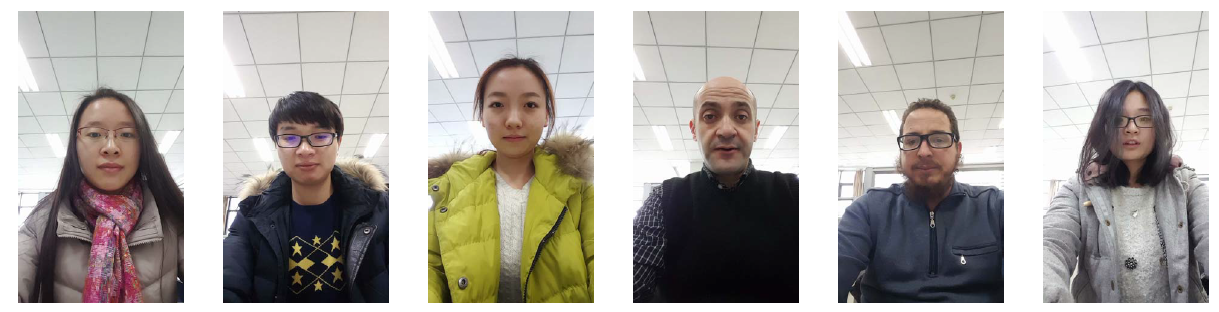
\includegraphics[width=\linewidth]{oulureal}}
 	\caption{نمونه‌های واقعی در دیتاست OULU \cite{boulkenafet2017oulu} }
 	\label{fig:oulureal}
 \end{figure}
 
 
  \begin{figure}[h]
 	\centerline{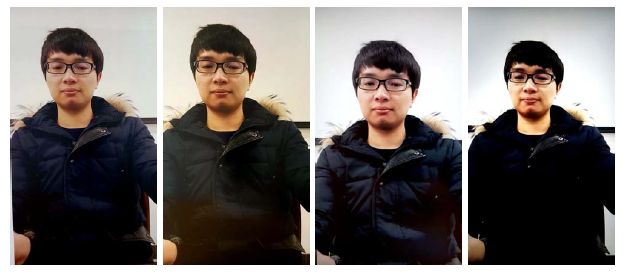
\includegraphics[width=\linewidth]{oulufake}}
 	\caption{نمونه‌های تقلبی در دیتاست OULU \cite{boulkenafet2017oulu} }
 	\label{fig:oulufake}
 \end{figure}
 
همچنین در این دیتاست برای گزارش دقت چهار پروتکل مختلف به‌منظور ارزیابی قابلیت تعمیم‌پذیری مدل ارائه شده در حالت‌های مختلف پیشنهاد شده‌است. پروتکل اول تنوع نشست را در دقت مدل بررسی می‌کند، بدین صورت که مدل باید روی داده‌های دو نشست از سه نشست آموزش ببیند و ارزیابی روی نشست سوم خواهد بود. در پروتکل دوم روی یک نوع از حمله کاغذ چاپ شده و یک نوع حمله‌ی بازپخش آموزش انجام می‌شود و در ارزیابی از نوع دیگر حمله باز پخش و کاغذ چاپ‌شده استفاده می‌شود تا تعمیم پذیری مدل روی حمله از ابزار دیده نشده بررسی شود. در پرتوکل سوم روی 5 نوع دوربین تلفن همراه از شش نوع آموزش انجام می‌شود و روی نوع ششم ارزیابی صورت می‌گیرد که این حالت برای بررسی قابلیت تعمیم پذیری روی نوع سنسور تصویر برداری دیده نشده انجام می‌گردد. پروتکل چهارم هر سه نوع پرتکل قبلی در هم ادغام می‌شوند تا اثر تنوع نشست، تنوع دوربین و تنوع نوع حمله ملاحظه شود.
\subsection{دیتاست SIW}
در دیتاست SIW
\cite{liu2018learning}
از 165 شخص مختلف برای تصویربرداری استفاده شده است. برای تصویربرداری از دو نوع دوربین با کیفیت استفاده شده است. در نمونه‌های واقعی تصویر برداری با فواصل مختلف دوربین تا کاربر انجام شده است تا تنوع فاصله کاربر با دوربین را پوشش دهد. همچنین از کاربر خواسته شده است که حالات مختلف چهره را به خود بگیرد و صورت خود را حرکت بدهد. این موجب تنوع در زاویه چهره نسب به دوربین و تنوع حالات چهره شده است. همچنین شرایط نورپردازی مختلف در این دیتاست دیده شده است. از دو نوع چاپگر برای حمله کاغذ چاپ‌شده استفاده شده‌است و از کاربر خواسته شده‌است که در دو حالت کاغذ را ثابت نگه دارد و آن را حرکت بدهد. همچنین از تبلت و دو نوع گوشی و صفحه نمایش‌گر رایانه برای حمله بازپخش استفاده شده است. نمونه‌های این دیتاست در  شکل 
\ref{fig:siw}
قابل مشاهده است. 
  \begin{figure}[h]
	\centerline{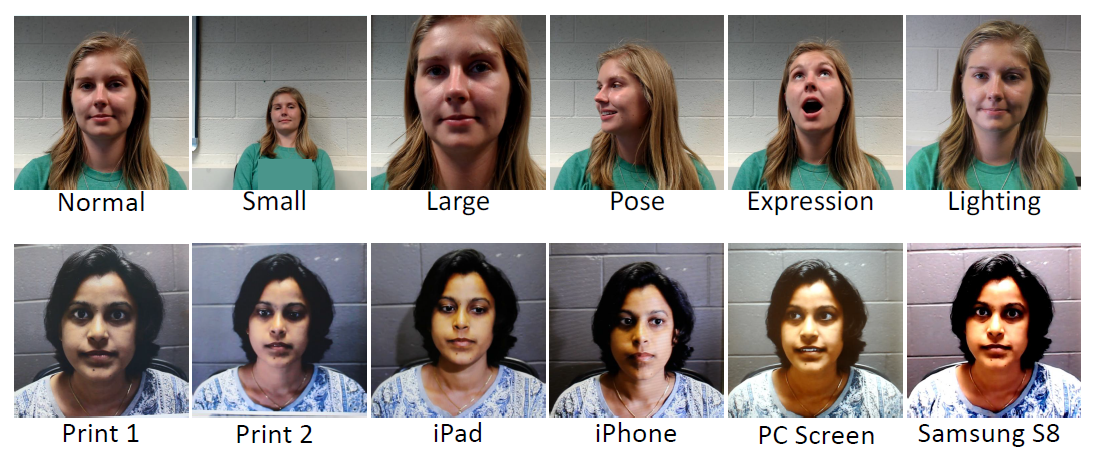
\includegraphics[width=\linewidth]{siw}}
	\caption{نمونه‌های از دیتاست SIW \cite{liu2018learning} }
	\label{fig:siw}
\end{figure}

این دیتاست دارای سه نوع پروتکل مختلف برای ارزیابی است. در پروتکل اول تنها از 60 فریم اول هر ویدئو برای آموزش استفاده می‌شود و از تمامی فریم‌های ویدیوهای تست برای ارزیابی استفاده می‌شود. از آنجا که در فریم‌های ابتدایی ویدئو کاربر صورت خود را حرکت نمی‌دهد این پروتکل به ارزیابی تغییر حالت چهره می‌پردازد. در پروتکل دوم از سه نوع حمله بازپخش استفاده می‌شود و روی حمله چهارم بازپخش ارزیابی می‌شود تا اثر تنوع ابزار حمله در بازپخش بررسی شود. در پروتکل سوم از یکی از انواع حمله بازپخش یا چاپ برای آموزش استفاده می‌شود و از نوع حمله دیگر برای تست استفاده می‌شود که هدف آن ارزیابی نوع حمله دیده نشده است. 





 











 












